\documentclass{beamer}
\usepackage[english]{babel}
\usepackage{graphicx}
\usepackage{hyperref}

\setbeamertemplate{navigation symbols}{}

\title[PL3GA Visualisation]{Visualization of the projective geometry for geometric algebra}
\subtitle{Final Presentation}
\author{Patrick de Kok}
\institute{Supervisor: Leo Dorst}
\date{June 28, 2012}

%% Math type specifying fonts
\newcommand{\V}[1]{\ensuremath{\mathbf{#1}}}
\newcommand{\s}[1]{\ensuremath{\mathcal{#1}}}

%% GA operators
\newcommand{\gp}{\ensuremath{\;}}
\newcommand{\gpi}{\ensuremath{\mathbin{/}}}
\newcommand{\lcont}{\ensuremath{\mathbin{\rfloor}}}
\newcommand{\rcont}{\ensuremath{\mathbin{\lfloor}}}
\newcommand{\dotp}{\ensuremath{\mathbin{\cdot}}}
\newcommand{\inverse}[1]{\ensuremath{#1^{-1}}}
\newcommand{\dual}[1]{\ensuremath{#1^\ast}}
\newcommand{\undual}[1]{\ensuremath{#1^{-\ast}}}
\newcommand{\edotp}{\ensuremath{\mathbin{\dotp_\mathbb{E}}}}
\newcommand{\elcont}{\ensuremath{\mathbin{\lcont_\mathbb{E}}}}
\newcommand{\ercont}{\ensuremath{\mathbin{\rcont_\mathbb{E}}}}
\newcommand{\edual}[1]{\ensuremath{#1 \lcont \inverse{\epseudo}}}
\newcommand{\eundual}[1]{\ensuremath{#1 \lcont \epseudo}}
%\newcommand{\edual}[1]{\ensuremath{#1^\bigstar}}
%\newcommand{\eundual}[1]{\ensuremath{#1^{-\bigstar}}}
\newcommand{\norm}[1]{\ensuremath{\left\|#1\right\|}}

\DeclareMathOperator{\pluckerid}{\Omega_q}
\DeclareMathOperator{\pluckerbilin}{\Omega}
\DeclareMathOperator{\Em}{Em}
\DeclareMathOperator{\grade}{\mathtt{grade}}
\newcommand{\pdual}[1]{\ensuremath{#1^\natural}}

\newcommand{\heq}{\ensuremath{\mathbin{=_{H}}}} % Homogeneous equality

%% Pl\"ucker notation
\newcommand{\plucker}[2]{\ensuremath{\{#1 \mathbin{:} #2\}}}
%\newcommand{\pluckerpoint}[2]{\ensuremath{(#1 \mathbin{:} #2)}}
%\newcommand{\pluckerplane}[2]{\ensuremath{[#1 \mathbin{:} #2]}}

%% Math-like symbols
\newcommand{\reals}{\ensuremath{\mathbb{R}}}
\newcommand{\en}{\ensuremath{\mathbin{\mbox{and}}}}
\newcommand{\of}{\ensuremath{\mathbin{\mbox{or}}}}
\newcommand{\eql}{\ensuremath{\Leftrightarrow}}

%% Math constants and shorthands
\newcommand{\pline}{\ensuremath{\ell}}
\newcommand{\rline}{\ensuremath{\ell_o}}
\newcommand{\iline}{\ensuremath{\ell_\infty}}
\newcommand{\screw}{\ensuremath{s}}

\newcommand{\ez}{\ensuremath{e_0}}
\newcommand{\ee}{\ensuremath{\V{e}_1}}
\newcommand{\et}{\ensuremath{\V{e}_2}}
\newcommand{\ed}{\ensuremath{\V{e}_3}}
\newcommand{\eze}{\ensuremath{e_{01}}}
\newcommand{\ezt}{\ensuremath{e_{02}}}
\newcommand{\ezd}{\ensuremath{e_{03}}}
\newcommand{\etd}{\ensuremath{e_{23}}}
\newcommand{\ede}{\ensuremath{e_{31}}}
\newcommand{\eet}{\ensuremath{e_{12}}}
\newcommand{\epseudo}{\ensuremath{\V{I}_3}}
\newcommand{\hpseudo}{\ensuremath{\ez\V{I}_3}}

\newcommand{\ap}{\ensuremath{a_{+}}}
\newcommand{\am}{\ensuremath{a_{-}}}
\newcommand{\bp}{\ensuremath{b_{+}}}
\newcommand{\bm}{\ensuremath{b_{-}}}
\newcommand{\cp}{\ensuremath{c_{+}}}
\newcommand{\cm}{\ensuremath{c_{-}}}

%% Text symbols
\newcommand{\newterm}{$^\dagger$}

\newcommand{\ega}{\texttt{e3ga}}
\newcommand{\pga}{\texttt{p3ga}}
\newcommand{\cga}{\texttt{c3ga}}
\newcommand{\cbga}{\texttt{c5ga}}
\newcommand{\iga}{\texttt{i2ga}}
\newcommand{\lga}{\texttt{l3ga}}

%% Setting color definitions
\definecolor{nicered}{rgb}{0.6, 0, 0.24}
\definecolor{nicegreen}{rgb}{0.0, 0.5, 0.24}
\definecolor{niceblue}{rgb}{0, 0.4, 1}
\definecolor{gray}{rgb}{0.2, 0.2, 0.2}
\definecolor{lightgray}{rgb}{0.4, 0.4, 0.4}

\newtoggle{draft}

\AtEndPreamble{
  \iftoggle{draft}{
    \hypersetup{
      colorlinks=true, 
      urlcolor=nicegreen,
      linkcolor=niceblue,
      citecolor=nicered,
    }
    \newcommand{\comment}[1]{\colorbox{red}{\bfseries\color{white}#1}}
    \newcommand{\TODO}[1]{\colorbox{niceblue}{\bfseries\color{white}TODO: #1}}
    \newcommand{\askLeo}[1]{\colorbox{yellow}{\bfseries Leo: #1}}
  }{
    \hypersetup{
      colorlinks=true,
      urlcolor=gray,
      linkcolor=gray,
      citecolor=lightgray,}
    \newcommand{\comment}[1]{}
    \newcommand{\TODO}[1]{}
    \newcommand{\askLeo}[1]{}
    }}

\makeatletter
%% Provide \Autoref; the \autoref with a printed capital
\def\figureautorefname{figure}
\def\tableautorefname{table}
\def\partautorefname{part}
\def\appendixautorefname{appendix}
\def\equationautorefname{equation}
\def\AMSautorefname{equation}
\def\theoremautorefname{theorem}
\def\Autoref#1{%
  \begingroup
  \edef\reserved@a{\cpttrimspaces{#1}}%
  \ifcsndefTF{r@#1}{%
    \xaftercsname{\expandafter\testreftype\@fourthoffive}
      {r@\reserved@a}.\\{#1}%
  }{%
    \ref{#1}%
  }%
  \endgroup
}
\def\testreftype#1.#2\\#3{%
  \ifcsndefTF{#1autorefname}{%
    \def\reserved@a##1##2\@nil{%
      \uppercase{\def\ref@name{##1}}%
      \csn@edef{#1autorefname}{\ref@name##2}%
      \autoref{#3}%
    }%
    \reserved@a#1\@nil
  }{%
    \autoref{#3}%
  }%
}

%% Commands for the title page.
% The title page needs the following data to be shown correctly:
% - \title
% - \subtitle (optional)
% - \studentid
% - \ects
% - \programme
% - \programmeaddress
% - \supervisor
% - \supervisoraddress
% - \finaldate or \date
\def\title#1{\gdef\@title{#1}}
\def\subtitle#1{\gdef\@subtitle{#1}}
\def\studentid#1{\gdef\@studentid{#1}}
\def\ects#1{\gdef\@ects{#1}}
\def\programme#1{\gdef\@programme{#1}}
\def\programmeaddress#1{\gdef\@programmeaddress{#1}}
\def\supervisor#1{\gdef\@supervisor{#1}}
\def\supervisoraddress#1{\gdef\@supervisoraddress{#1}}
\def\finaldate#1{\gdef\@finaldate{#1}}

\renewcommand{\maketitle}{
\begin{titlepage}
\begin{center}

\vspace{2.5cm}

\begin{Huge}
\@title
\end{Huge}
\rule{\linewidth}{0.1pt}

\ifdef{\@subtitle}{
\begin{large}
\@subtitle
\end{large}}{}

\vspace{1.5cm}

\@author\\
\@studentid

\vspace{1.5cm}

% [DO NOT CHANGE]
Bachelor thesis\\
% [CHANGE] Whether your Bachelor thesis is 6 ECTS (regular) or 9 ECTS (Honours
% programme).
Credits: \@ects{}EC

\vspace{0.5cm}

% [DO NOT CHANGE] The name of the educational programme.
\@programme

\vspace{0.25cm}

% [DO NOT CHANGE] The addess of the educational programme.
\@programmeaddress

\vspace{4cm}

\emph{Supervisor}\\
% [CHANGE] The name of your supervisor. Include the titles of your supervisor,
% as well as the initials for *all* of his/her first names.
\@supervisor

\vspace{0.25cm}

% [CHANGE] The address of the institute at which your supervisor is working.
% Be sure to include (1) institute (is appropriate), (2) faculty (if
% appropriate), (3) organisation name, (4) organisation address (2 lines).
\@supervisoraddress

\vspace{1.5cm}

% [CHANGE] The date at which you will finalize and submit your thesis.
\ifdef{\@finaldate}{\@finaldate}{\@date}

\end{center}
\addtocounter{page}{-1}
\end{titlepage}

}
\makeatother

\newcommand{\supcite}[1]{\textsuperscript{\cite{#1}}}
\newcommand{\pro}{\structure{\textbf{+}}}
\newcommand{\con}{\structure{\textbf{--}}}

\begin{document}
\begin{frame}
  \titlepage
\end{frame}

\begin{frame}{Project description}
    Extend a \alert<3>{graphical calculator} of \alert<1>{geometric algebra} to model the \alert<2>{projective geometry of lines}.

    \only<+>{
      \begin{itemize}
        \item Much like linear algebra, but has structure preserving operations
        \item Outer product $\wedge$ to create subspaces
        \item Implementations are fast~\supcite{Fontijne2003}
      \end{itemize}
    }
    \only<+>{
      \begin{itemize}
        \item Useful for computer vision, graphics, robotics\ldots
        \item Pl\"ucker coordinates: 3D lines are 6D null vectors
          \begin{itemize}
            \item Representation is homogeneous
          \end{itemize}
        \item Recently found an operational model for geometric algebra~\supcite{Hongbo}
      \end{itemize}
    }
    \only<+>{
      \begin{center}
        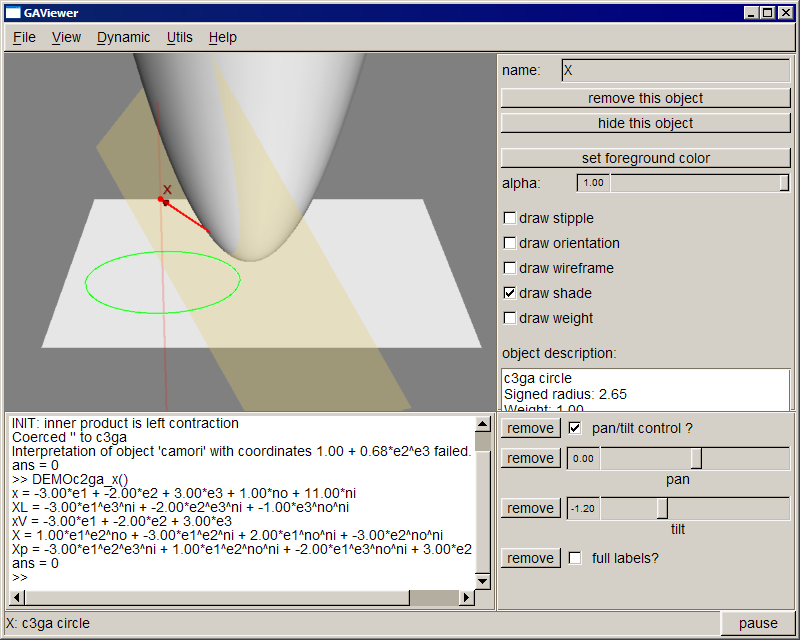
\includegraphics[width=0.7\textwidth]{gaviewer}

        \href{http://geometricalgebra.net/gaviewer_download.net}{\texttt{http://geometricalgebra.net} $\to$ Downloads $\to$ GAViewer}
      \end{center}
    }
\end{frame}

\begin{frame}{Approach}
  \begin{enumerate}
    \item Understand Pl\"ucker model for GA
    \item Explore part of the representation space
      \begin{itemize}
        \item Geometric interpretation of subspaces
        \item Compute location, stance, weight, orientation
      \end{itemize}
    \item Extend GAViewer
      \begin{itemize}
        \item Recognise geometric type of input
        \item Implement drawing routines
      \end{itemize}
  \end{enumerate}
\end{frame}

\begin{frame}{Pl\"ucker model}
  Really new to GA community
  \begin{itemize}
    \item Original article defines metric and vector space $\mathbb{R}^{3,3}$
    \item No further connection with model in other algebras shown
    \item No further articles on Pl\"ucker model for GA
  \end{itemize}
  \bigskip 
  \ldots but well known for other algebras
  \begin{itemize}
    \item Big difference in vocabulary
    \item Less focus on subspace nature
    \item Some GA concepts not well defined in LA
  \end{itemize}
\end{frame}

\begin{frame}{But first\ldots}
  Recall homogeneous model
  \begin{itemize}
    \item Extends Euclidean directions $\ee, \et, \ed$ with point $\ez$
    \item Point $p = \V{p} + \lambda \ez$ has location $\frac{p}{\ez \dotp p}$ and weight $\lambda$
    \item Directions have weight $\lambda = 0$, so location is at infinity
    \item Average of two points gives new point
  \end{itemize}
\end{frame}

\begin{frame}{Lines defined}
  \begin{columns}
    \begin{column}{5cm}
      Define line $L$ by a point $p$ and direction $\V{d}$:
      \begin{equation*}
        L  = p \wedge \V{d}
      \end{equation*}
      $\lambda L$ only differs in weight and orientation
    \end{column}
    \begin{column}{5cm}
      \begin{center}
        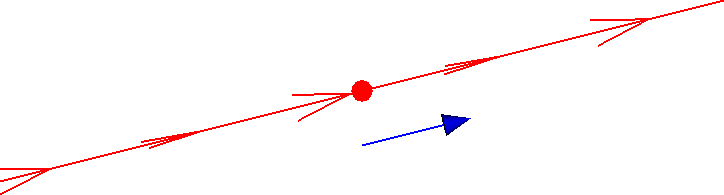
\includegraphics[width=5cm]{line}
      \end{center}
    \end{column}
  \end{columns}
\end{frame}

\begin{frame}{Pl\"ucker space}
  \begin{columns}
    \begin{column}{5cm}
      Basis of our vector space $\reals^{3,3}$: 
      \begin{equation*}
        \begin{array}{l}
          \left. \begin{array}{l}
            \ez\wedge\ee = \eze \\
            \ez\wedge\et = \ezt \\
            \ez\wedge\ed = \ezd
          \end{array} \right\} \mbox{Finite lines}
          \\
          \left. \begin{array}{l}
            \et\wedge\ed = \etd \\
            \ed\wedge\ee = \ede \\
            \ee\wedge\et = \eet
          \end{array} \right\} \mbox{Lines at infinity}
        \end{array}
      \end{equation*}
      %With dot product:
      %\begin{equation*}
      %  \eze \dotp \etd = \ezt \dotp \ede = \ezd \dotp \eet = 1
      %\end{equation*}
    \end{column}
    \begin{column}{5cm}
      \begin{center}
        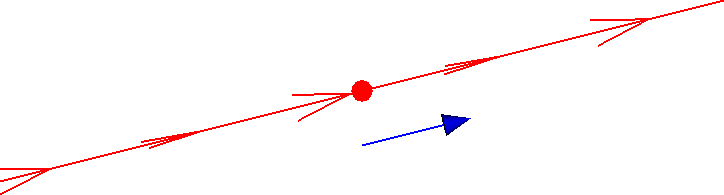
\includegraphics[width=5cm]{line}

        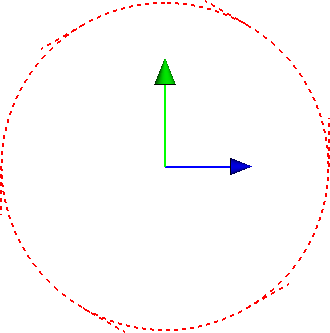
\includegraphics[width=3cm]{idealline}
      \end{center}
    \end{column}
  \end{columns}
\end{frame}

\begin{frame}{Lines are screws}
  \begin{columns}
    \begin{column}{7cm}
      Screws are general basic geometric entity
      \begin{itemize}
        \item Finite lines only translate
        \item Lines at infinity only rotate
      \end{itemize}
      \ldots but we only look at subspaces of lines
    \end{column}
    \begin{column}{3cm}
      \begin{center}
        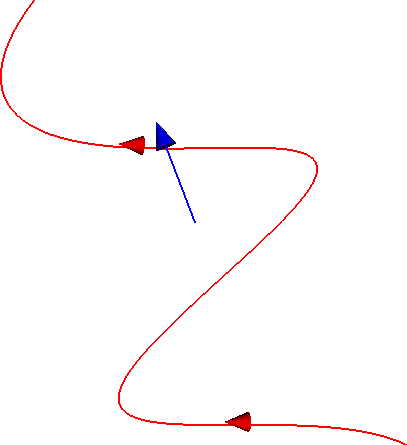
\includegraphics[width=3cm]{screw}
      \end{center}
    \end{column}
  \end{columns}
\end{frame}

\begin{frame}{Combining lines}
  Geometrical different cases
  \begin{enumerate}
    \item 2 intersecting and parallel lines
    \item 2 skew lines
    \item 3 lines intersect in 1 point
    \item 3 lines intersect in different points
    \item 1 line intersects 2 other lines
    \item 3 skew lines
  \end{enumerate}
\end{frame}

\begin{frame}{Pencils of lines}
  \begin{columns}
    \begin{column}{5cm}
      Two lines $\ell_1, \ell_2$ intersect

      \bigskip

      Parallel lines intersect in point at infinity!
    \end{column}
    \begin{column}{5cm}
      \begin{center}
      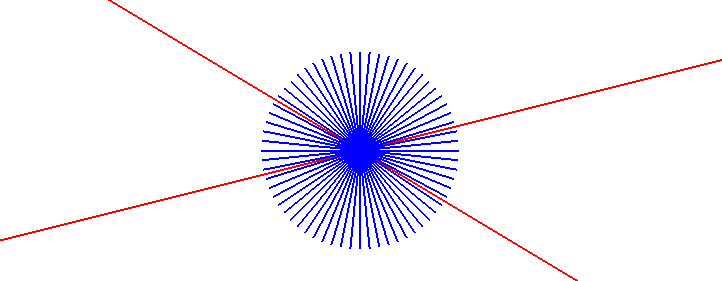
\includegraphics[width=5cm]{pencil1}

      
\includegraphics[width=5cm]{pencil2}

      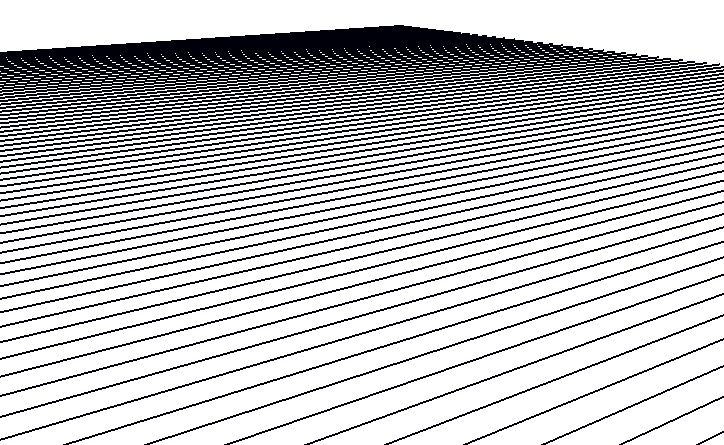
\includegraphics[width=5cm]{pencil3}
    \end{center}
    \end{column}
  \end{columns}
\end{frame}

\begin{frame}{Line pair}
  \begin{columns}
    \begin{column}{5cm}
      When $\ell_1, \ell_2$ don't intersect, $\ell_1 \wedge \ell_2$ only contains those two lines

      \bigskip

      Dual of $\ell_1 \wedge \ell_2$ contains all lines intersecting both 
    \end{column}
    \begin{column}{5cm}
      \begin{center}
        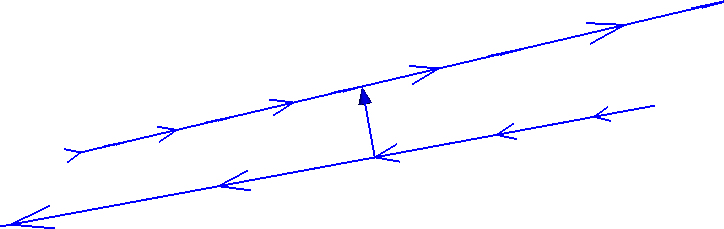
\includegraphics[width=5cm]{linepair1}

        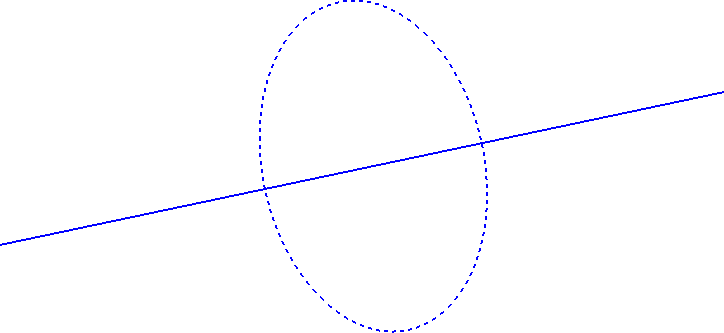
\includegraphics[width=5cm]{linepair2}

        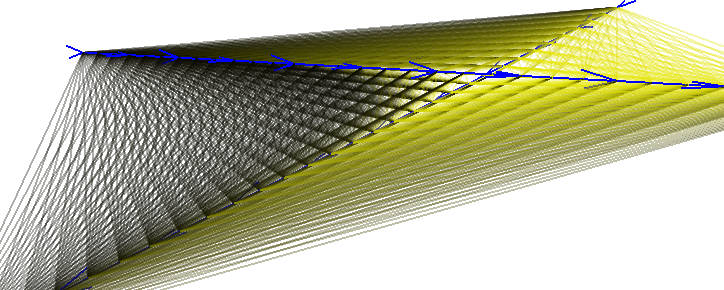
\includegraphics[width=5cm]{linepair3}
      \end{center}
    \end{column}
  \end{columns}
\end{frame}

\begin{frame}{Finite and infinite points}
  \begin{columns}
    \begin{column}{5cm}
      Two interpretations:
      \begin{enumerate}
        \item All lines intersecting in a point
        \item The point of intersection
      \end{enumerate}

      \bigskip

      Three parallel lines intersect in a pair of points
    \end{column}
    \begin{column}{5cm}
      \begin{center}
        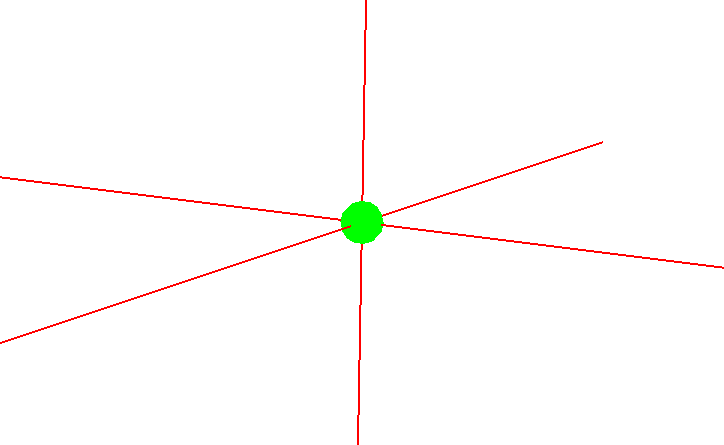
\includegraphics[width=5cm]{point1}

        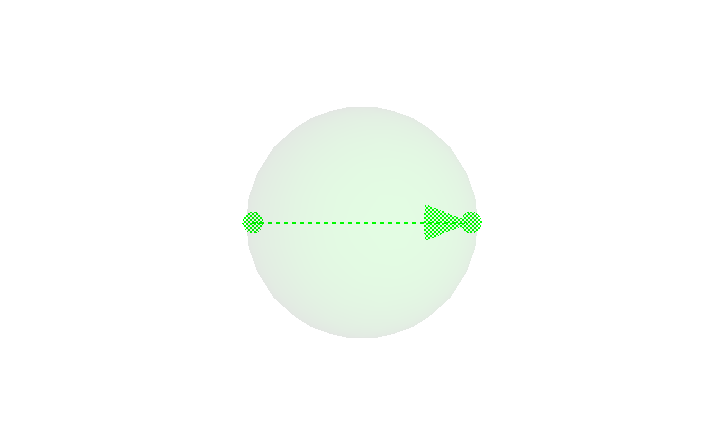
\includegraphics[width=5cm]{point2}
      \end{center}
    \end{column}
  \end{columns}
\end{frame}

\begin{frame}{Planes}
  \begin{columns}
    \begin{column}{5cm}
      If 3 lines intersect in 3 points, the linear combination is their common plane
      \bigskip
      Only 1 infinite plane, corresponds to Euclidean space
    \end{column}
    \begin{column}{5cm}
      \begin{center}
        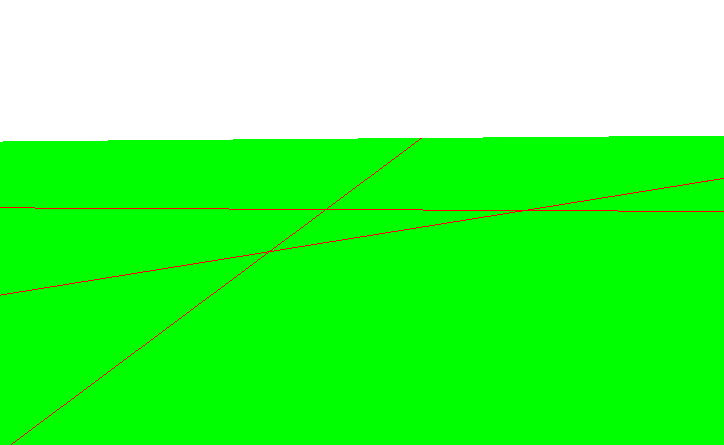
\includegraphics[width=5cm]{plane1}

        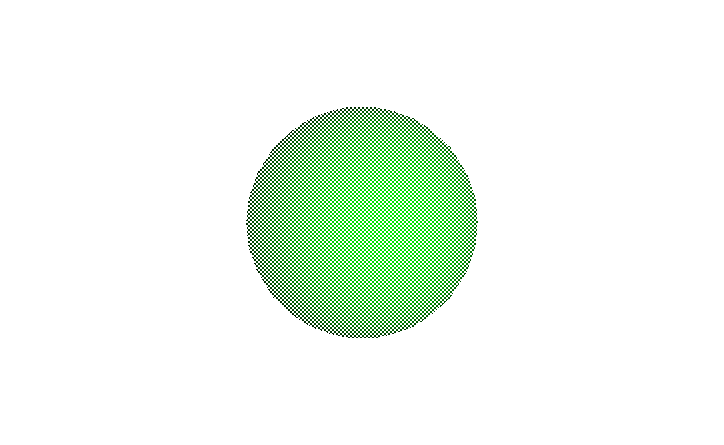
\includegraphics[width=5cm]{plane2}
      \end{center}
    \end{column}
  \end{columns}
\end{frame}

\begin{frame}{Pair of pencils}
  \begin{columns}
    \begin{column}{5cm}
      Combines the set of lines of $\ell_1 \wedge \ell_2$, $\ell_2 \wedge \ell_3$ and $\ell_3 \wedge \ell_1$
    \end{column}
    \begin{column}{5cm}
      \begin{center}
        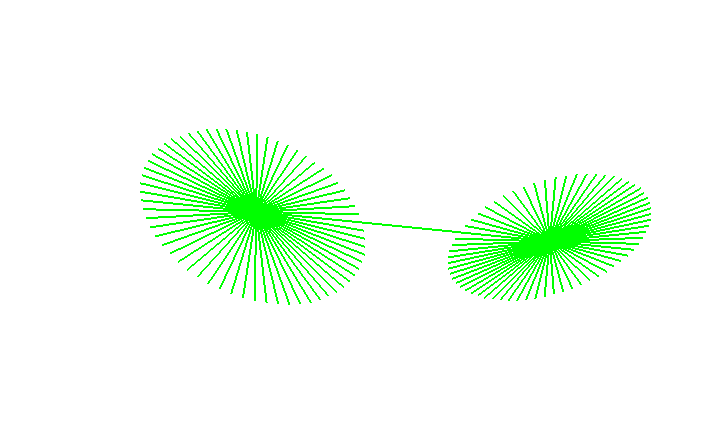
\includegraphics[width=5cm]{cwpencil}
      \end{center}
    \end{column}
  \end{columns}
\end{frame}

\begin{frame}{Regulus}
  \begin{columns}
    \begin{column}{5cm}
      Three skew lines

      \bigskip

      Not implemented; unclear how to parameterize the set of lines
    \end{column}
    \begin{column}{5cm}
      \begin{center}
        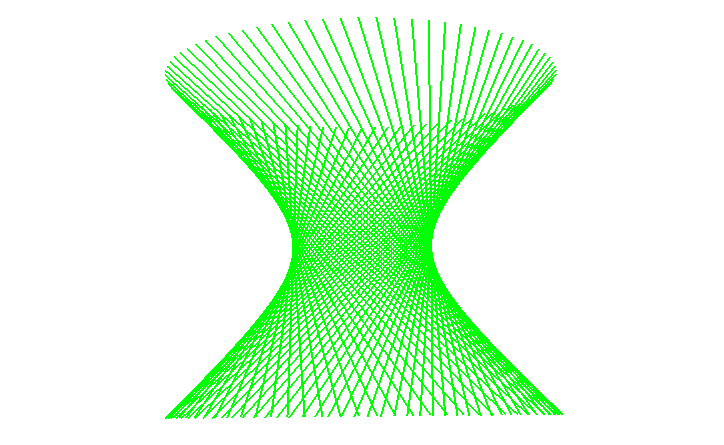
\includegraphics[width=5cm]{regulus1}

        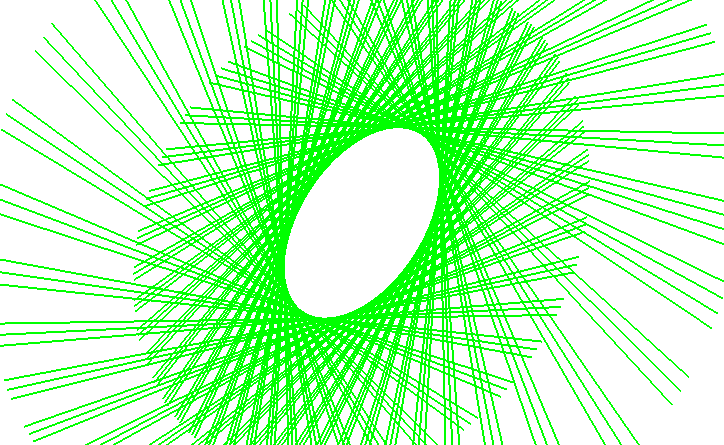
\includegraphics[width=5cm]{regulus2}
      \end{center}
    \end{column}
  \end{columns}
\end{frame}

\begin{frame}{Extending GAViewer}
  Easily done:
  \begin{itemize}
    \item Generate GA code for Pl\"ucker model
    \item Only need to implement classification, visualization, what to do on mouse drag
  \end{itemize}
  
  \ldots if you know how.
  \begin{itemize}
    \item Little documentation on where to put new code
  \end{itemize}
\end{frame}

\begin{frame}{Results}
  Much is done
  \begin{enumerate}
    \item Show correspondencies between Pl\"ucker model for LA and GA
    \item Computed 4 geometrically important features of almost all line-subspaces
    \item Implemented classifications and visualizations
  \end{enumerate}
  But much more can be done
  \begin{enumerate}
    \item Compute features of reguli
    \item Compute combinations of screws
    \item Connections with other models?
    \item Ellipse representation?
    \item Pl\"ucker model for $\reals^2$?
  \end{enumerate}
\end{frame}

\begin{frame}{Questions}
  \begin{center}
    %{\Large\structure{Questions}}
    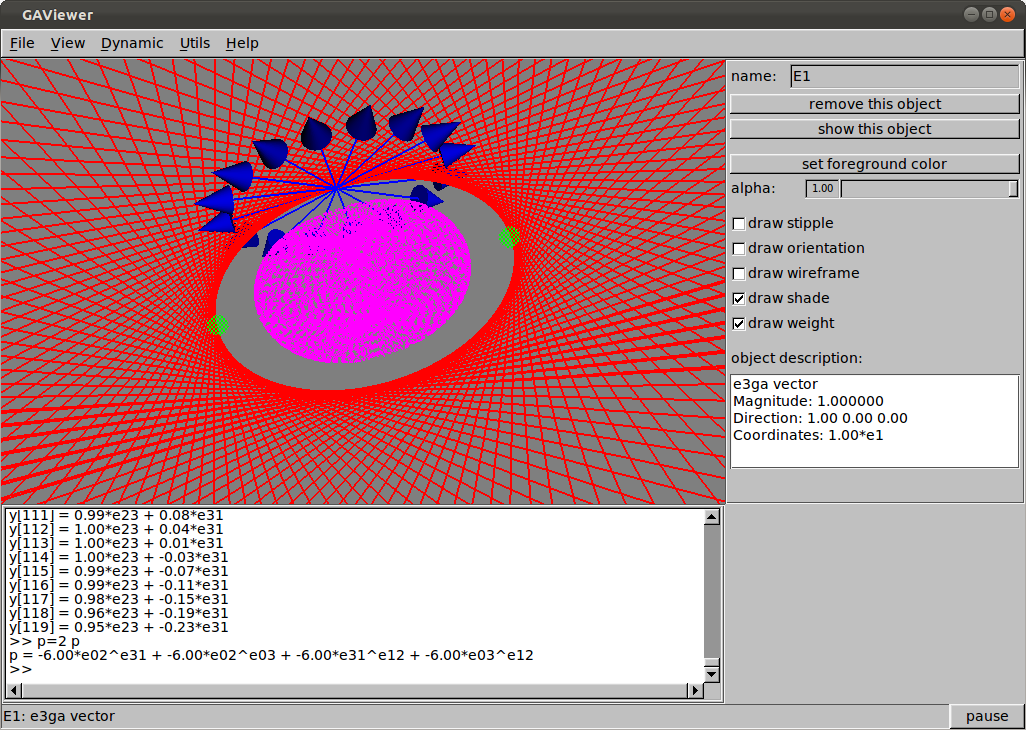
\includegraphics[width=1\textwidth]{gaviewer3}
  \end{center}
\end{frame}

\begin{frame}{Bibliography}
  \bibliographystyle{plainnat}
  \bibliography{../thesis/citations}
\end{frame}

\end{document}
